\begin{titlepage}
\begin{center}

\vspace*{0.5cm}
\HUGE \textbf{分科化學第二冊}\\
\vspace{1cm}
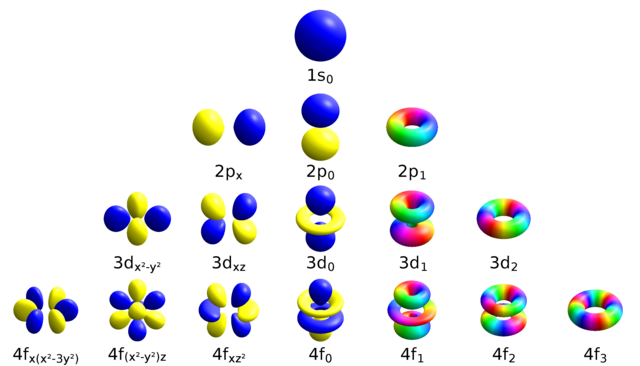
\includegraphics[width=15cm]{Atomic_orbitals_spdf_m-eigenstates_and_superpositions.png}\\[1cm]
\HUGE \textbf{軌域}\\
\vfill

\large
章節關鍵字

\begin{tabular}{l}
氫原子模型 \\
芮得柏常數 $R_H = 1.097\times10^{-2}\,\mathrm{nm^{-1}}$ \\
萊曼 / 巴耳末 / 帕申 / 布拉克特 系列 \\
量子數 \\
$s,p,d,f$ 軌域 \\
\end{tabular}
\\[1cm]
\Large charlie.note.os\\[0.5cm]


\end{center}

\end{titlepage}